\documentclass[11pt, oneside, a4paper]{article}
%\documentclass[11pt, oneside, a4paper, twocolumn]{article}
\usepackage[utf8]{inputenc}
\usepackage[english,russian]{babel}
\edef\restoreparindent{\parindent=\the\parindent\relax}
\usepackage{parskip}
\restoreparindent
\usepackage{indentfirst}
\setlength{\topmargin}{-1in}
\setlength{\textheight}{10.2in}
\setlength{\textwidth}{7.1in} 
\setlength{\footskip}{0.6in}
\setlength{\oddsidemargin}{-0.3in}
\pretolerance=150
\newcommand{\cm}[1]{\par\textbf{{#1}}\par}
\usepackage[ backend=bibtex, natbib=true, style=numeric, sorting=none]{biblatex}
\addbibresource{../library.bib}

\usepackage{csquotes}
\usepackage[svgnames]{xcolor}
\usepackage[colorlinks=true, citecolor=Black, linkcolor=Black, urlcolor=Black]{hyperref}
\usepackage{bookmark}
\usepackage{mathtools}
\usepackage{float}
\usepackage{subcaption}
\usepackage{svg}
\usepackage{algorithm2e}
\begin{document}
\selectlanguage{russian}
\title{Оценка влияния шага интегрирования на результат расчета гибкой стержневой нити}
\author{Oleksandr Hubanov\\
Vilnius Gediminas Technical University}
\maketitle

\chapter*{Introduction}
%Введение и постановка задачи 
The mitral valve, also known as the bicuspid valve or left atrioventricular
valve, is a valve with two flaps in the heart, that lies between the left atrium
and the left ventricle. The mitral valve and the tricuspid valve are known
collectively as the atrioventricular valves because they lie between the atria
and the ventricles of the heart.
\begin{figure}[H]
  \centering
  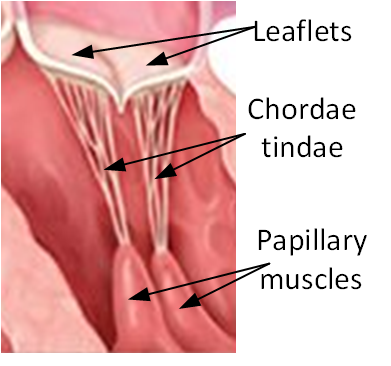
\includegraphics[width=0.4\textwidth]{./fig/mt.png}
    \caption{Mitral valve structure}
    \label{fig:MT}
\end{figure}
Mechanical properties
Chordae:
L ~ 0,025 m (length)
d ~ 0,001 m (diameter)
$\rho$ = 1040 kg/m3 (density)
E = 2000 N/m (stiffness)
Poisson's ratio of 0.49

Leaflets:
E = 2.0E6 MPa (Anterior leaflet)
E = 1.0E6 MPa (Posterior leaflet)
$\rho$ = 1.06E3 kg/m3 
Poisson’s ratio 0.49 
\par
Mitral valve has cyclic working conditions. Example of such you can see on
figure \ref{fig:workMT}.
\begin{figure}[H]
  \centering
  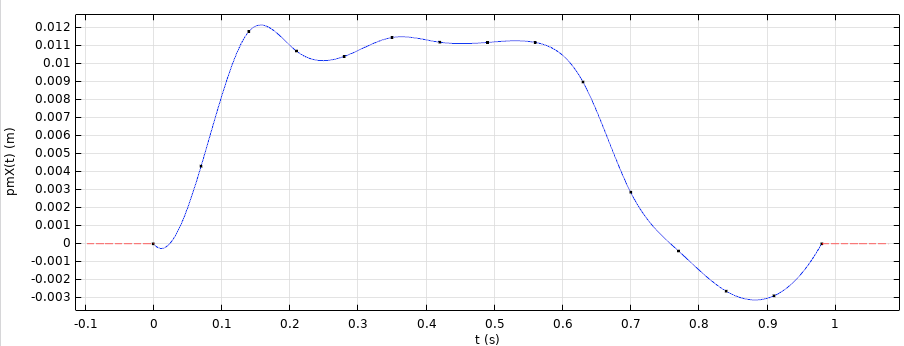
\includegraphics[width=0.8\textwidth]{./fig/workMT.png}
    \caption{Displacement of papillary muscle over cardiac cycle}
    \label{fig:workMT}
\end{figure}
 In normal conditions, blood flows through an open mitral valve during diastole
with contraction of the left atrium, and the mitral valve closes during systole
with contraction of the left ventricle. The valve opens and closes because of
pressure differences, opening when there is greater pressure in the left atrium
than ventricle, and closing when there is greater pressure in the ventricle than
atrium. In abnormal conditions, blood may flow backwards through the valve
(mitral regurgitation) or the mitral valve may be narrowed (mitral stenosis).
Rheumatic heart disease often affects the mitral valve; the valve may also
prolapse with age, and be affected by infective endocarditis. The mitral valve
is named after the mitre of a bishop, which resembles its flaps.
\begin{figure}[H]\label{fig:workingMT}      
  \centering
  \begin{subfigure}[b]{0.4\textwidth}\label{fig:openMT}
    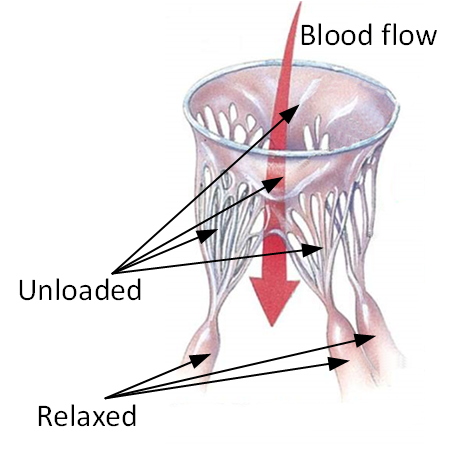
\includegraphics[width=\textwidth]{./fig/openMT.png}
      \caption{Opened state of mitral valve}      
  \end{subfigure}
  ~
  ~ %add desired spacing between images, e. g. ~, \quad, \qquad, \hfill etc. 
    %(or a blank line to force the subfigure onto a new line)
  \begin{subfigure}[b]{0.4\textwidth}\label{fig:closedMT}  
    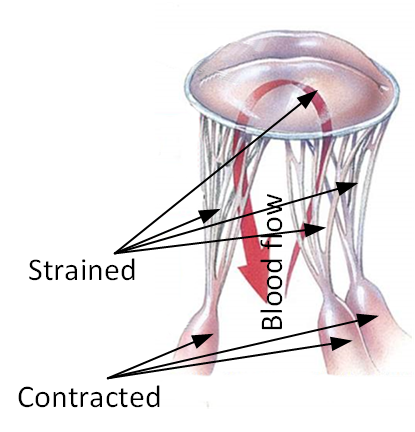
\includegraphics[width=\textwidth]{./fig/closedMT.png}
      \caption{Closed state of mitral valve}    
  \end{subfigure}
  \caption{Mitral valve working cycle}
\end{figure} 

Mitral valve prolapse (MVP) is a valvular heart disease characterized by the
displacement of an abnormally thickened mitral valve leaflet into the left
atrium during systole. By other words, it is a condition in which the two flaps
of the mitral valve doesn't close smoothly and evenly, but instead bulge
(prolapse) upward into the left atrium.\cite{Hayek2005a}
\begin{figure}[H]\label{fig:compareMT}
  \centering
  \begin{subfigure}[b]{0.4\textwidth}\label{fig:normalMT}
    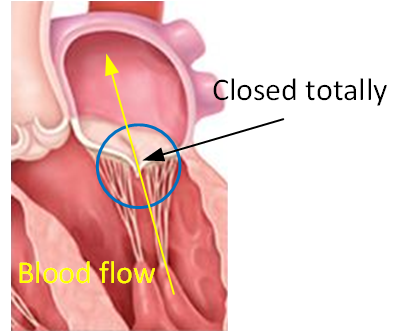
\includegraphics[width=\textwidth]{./fig/normalMT.png}
      \caption{Normal mitral valve}      
  \end{subfigure}
  ~
  ~ 
  \begin{subfigure}[b]{0.4\textwidth}\label{fig:prolapseMT}
    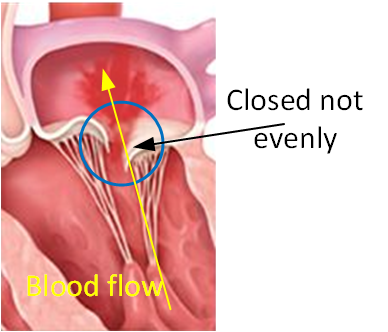
\includegraphics[width=\textwidth]{./fig/prolapseMT.png}
      \caption{Prolapse mitral valve}      
  \end{subfigure}
  \caption{Comparison of the normal valve and prolapse}      
\end{figure} 
Providing the surgeon with an anatomically and biomechanically accurate
computional model of a particular patient's mitral heart valve could enable
preoperative surgical planning and potentially improve surgical outcome.
Investigation behavior of biological tissue can be done by estimating movement
of it. Tissues of biological origin, usually had a weak structure and little
stiffness.
\par
%FEM explisit(abaqus) and MSM
Such physical structure imposes restrictions on the possible tools in the
measurement. Another possible problem is the limited number of measurement
attempts. Such limitations of physical measurements call into question the
possibility of such activities in general. An alternative to physical
experiments is the numerical simulation of these experiments. There are a large
number of different numerical modeling methods. All of them are derivatives of
Finite Element Method(FEM) and Discrete Element Method(DEM).
\par
While general finite-element studies are helpful for the evaluation and
development of MV repair surgery, patient-specific models are required for
individual therapy planning.
\cm{article 1}
The patient-specific mass-spring MV model uses a segmentation of 3D TEE images
for the initialization of a mass-spring model of the closed MV under systolic
pressure. An iterative approach is used to adjust the spring rest-length so that
the model can accurately simulate the shape of the closed MV under systolic
pressure. To simulate MV annuloplasty, the model can then be deformed, according
to the annuloplasty ring to be used, to create a prediction of the shape of the
closed MV after surgery.
\par
Based on the properties of the material of biological tissues and review of
existing projects, the most appropriate method is Mass - Spring modeling(MSM). This
method based on ideas of DEM and basic element here is very know in mechanic
simple one dimensional(1D) beam.\ref{eqn:sacdd}
\cm{have to show so pic about MSM, with explanation what is going on}
Computational complexity of MSM is much less compare to FEM-based methods,
because of less number of equations to integrate on each time step. This
important advantage and physics way have method describes basic element gave to
MSM very wide using in computer games for calculating reality-looks hair or
cloth movement in real time. Modelling by using MSM could be parallel calculated
on each time step.\cite{Rasmusson2008} \cite{Amorim2012}
\par
%В расчете целого клапана берется один стержень, существующие варианты расчетов всей системы и как в них рассчитывается хорда
\begin{figure}[H]\label{fig:pc1}
  \centering
  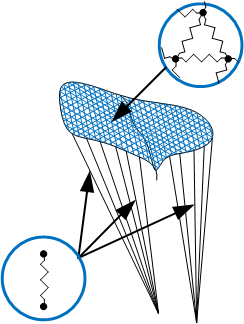
\includegraphics[width=0.2\textwidth]{./fig/pc1.png}
    \caption{Displacement of papillary muscle over cardiac cycle}    
\end{figure}
\begin{figure}[H]\label{fig:pc2}
  \centering
  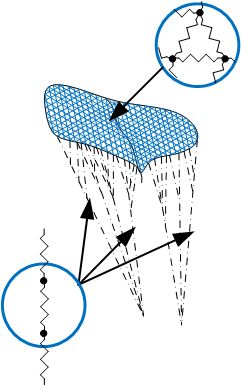
\includegraphics[width=0.2\textwidth]{./fig/pc2.png}
    \caption{Displacement of papillary muscle over cardiac cycle}    
\end{figure}
\begin{figure}[H]\label{fig:pc3}
  \centering
  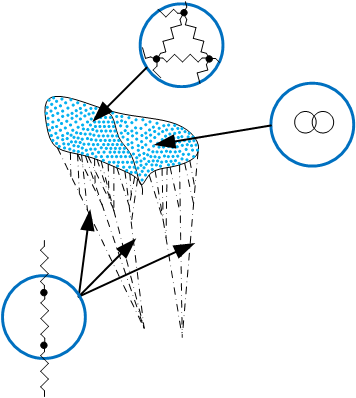
\includegraphics[width=0.3\textwidth]{./fig/pc3.png}
    \caption{Displacement of papillary muscle over cardiac cycle}    
\end{figure}
%Как движется кровь, описать механику (давление и скорость) сравнить преимущ от расчета давления от скорости
%Цель- сравнить одну стержень и систему
\input{whatIntegrMethodUsed.tex}
\input{comparingDeltaT.tex}
\input{resultsOverview.tex}

\printbibliography[title=List of literature]
\end{document}
